\documentclass[11pt,a4paper]{article}
 
\usepackage[utf8]{inputenc}
\usepackage[T1]{fontenc}
\usepackage{lmodern}
\usepackage[margin=2.2cm]{geometry}
\usepackage{booktabs}
\usepackage{listings}
\usepackage{xcolor}
\usepackage{hyperref}
\usepackage{enumitem}
\usepackage{amssymb}
\usepackage{titlesec}
\usepackage{array}
\usepackage{tikz}
\usetikzlibrary{arrows.meta, positioning}
 
\definecolor{codebg}{RGB}{246,246,248}
\definecolor{codekw}{RGB}{0,90,180}
\definecolor{codestr}{RGB}{160,50,50}
\definecolor{codegreen}{RGB}{30,120,60}
\definecolor{panelblue}{RGB}{40,90,160}
\definecolor{panelred}{RGB}{170,40,40}
\definecolor{panelgreen}{RGB}{40,130,70}
\definecolor{panelgray}{RGB}{90,90,90}
\definecolor{notebg}{RGB}{235,243,252}
 
\lstdefinestyle{code}{
  basicstyle=\ttfamily\footnotesize,
  backgroundcolor=\color{codebg},
  keywordstyle=\color{codekw}\bfseries,
  stringstyle=\color{codestr},
  commentstyle=\color{codegreen}\itshape,
  frame=single,
  rulecolor=\color{gray!50},
  breaklines=true,
  columns=fullflexible,
  keepspaces=true,
  showstringspaces=false,
  extendedchars=false,
  upquote=true,
}
\lstset{style=code}
 
\titleformat{\section}{\Large\bfseries\color{panelblue}}{\thesection}{0.6em}{}
\titleformat{\subsection}{\large\bfseries}{}{0pt}{}
 
\newcommand{\keyidea}[1]{%
  \par\smallskip\noindent\colorbox{notebg}{\parbox{\dimexpr\linewidth-2\fboxsep}{\small\textbf{Key idea.} #1}}\par\smallskip}
 
\hypersetup{colorlinks=true, linkcolor=panelblue, urlcolor=panelblue}
 
\title{\textbf{Concepts Behind the Secure SQL AI Agent}\\[4pt]
       \large A learning companion for version 0.2}
\author{}
\date{\today}
 
\begin{document}
\sloppy
\maketitle
\tableofcontents
\newpage
 
\section*{How to read this document}
 
Each section explains one idea and then points at the file where it lives.
If you are new to LLM agents, read in order. Sections~\ref{sec:pipeline}
and~\ref{sec:prompt} describe the whole request flow; Section~\ref{sec:cases}
walks through real bugs that were found and fixed in v0.2, which is the
fastest way to understand \emph{why} each check exists. Section~\ref{sec:quiz}
lets you test yourself.
 
% =====================================================================
\section{What ``an LLM agent'' actually means}
 
An LLM by itself is a text generator. You give it a prompt, you get text back.
An \emph{agent} adds three things on top:
 
\begin{enumerate}[leftmargin=*]
  \item \textbf{Context}: the model is given structured information about the
        world it reasons about. Here: the live database schema, including
        primary and foreign keys.
  \item \textbf{Tools}: the model's output is fed into real code that has
        effects. Here: a SQL parser, validators and an executor.
  \item \textbf{Control loop}: the model may be called again with the results
        of a previous attempt. Here: self-repair after a validation error.
\end{enumerate}
 
The agent is \emph{not} the model. The agent is the Python orchestration
around the model --- the pipeline in \texttt{app/agent.py}.
 
\begin{center}
\begin{tabular}{@{}ll@{}}
\toprule
\textbf{The LLM} & \textbf{The agent} \\
\midrule
Probabilistic text generator & Deterministic Python pipeline \\
Might hallucinate            & Enforces invariants \\
Cannot execute anything      & Executes only within policy \\
Its output is a proposal     & Trusts nothing, validates everything \\
\bottomrule
\end{tabular}
\end{center}
 
\keyidea{If the LLM is wrong, confused or manipulated, a well-designed agent
still refuses to run unsafe SQL. If the agent trusts the LLM, no amount of
model quality saves you.}
 
% =====================================================================
\section{Text-to-SQL: what can go wrong}
 
\textbf{Text-to-SQL} means translating a natural-language question into SQL.
These failure modes are not hypothetical; every one of them is handled by a
specific check in the project.
 
\subsection*{1. Hallucinated schema}
\begin{lstlisting}[language=SQL]
SELECT age FROM customers;   -- 'age' does not exist
\end{lstlisting}
Caught by schema validation against the live database, then fed back to the
model for repair.
 
\subsection*{2. Intent misclassification}
The user says ``clean up old orders''; the model writes a \texttt{DELETE}.
It is a \emph{write}, so it can only run after a human approves it.
 
\subsection*{3. A write disguised as a read}
\begin{lstlisting}[language=SQL]
WITH deleted AS (DELETE FROM users RETURNING id) SELECT * FROM deleted;
\end{lstlisting}
``Starts with WITH/SELECT, so it is safe'' is wrong. AST classification finds
the \texttt{Delete} node.
 
\subsection*{4. A write hidden inside another write}
\begin{lstlisting}[language=SQL]
WITH d AS (DELETE FROM customers RETURNING id)
INSERT INTO audit_ids (id) SELECT id FROM d;
\end{lstlisting}
The approval screen says \texttt{INSERT}, but every customer is deleted.
v0.2 rejects any write that contains a second data-modifying statement.
 
\subsection*{5. Multiple statements}
\begin{lstlisting}[language=SQL]
SELECT * FROM users; DROP TABLE users;
\end{lstlisting}
The parser reads the \emph{whole} string and rejects more than one statement.
 
\subsection*{6. Prompt injection from data}
A row can contain text like \emph{``ignore previous instructions''}. The agent
never sends row contents to the model --- only the schema shape --- so data
cannot become instructions.
 
\subsection*{7. Dangerous functions}
\texttt{pg\_read\_file}, \texttt{dblink}, \texttt{pg\_sleep},
\texttt{set\_config}, \texttt{query\_to\_xml} (which runs SQL stored in a
string) \dots{} are denied in \emph{every} statement type, not only SELECTs.
 
\subsection*{8. Silent data loss}
\begin{lstlisting}[language=SQL]
DELETE FROM orders;                                  -- no WHERE
DELETE FROM orders WHERE 1 = 1;                      -- WHERE that filters nothing
UPDATE products SET price = (SELECT max(price) FROM products WHERE id = 1);
\end{lstlisting}
All three touch every row. The third has a \texttt{WHERE}, but only inside the
sub-query. Section~\ref{sec:bounded} explains how the agent tells them apart.
 
\subsection*{9. The human makes it worse}
At the approval prompt the user can \emph{edit} the SQL. An edit is just as
untrusted as model output (Section~\ref{sec:edits}).
 
% =====================================================================
\section{Why regex cannot validate SQL}
 
\begin{lstlisting}[language=SQL]
/* comment */ SELECT * FROM users; DELETE FROM users;
WITH x AS (DELETE FROM users RETURNING id) SELECT * FROM x;
SELECT * INTO backup_users FROM users;         -- creates a table
SELECT * FROM users FOR UPDATE;                -- locks rows
\end{lstlisting}
 
All four are dangerous; three of them contain \texttt{SELECT} first.
To classify SQL correctly you need a parser that builds an
\textbf{Abstract Syntax Tree} (AST): a tree of typed nodes such as
\texttt{Select}, \texttt{Delete}, \texttt{Table}, \texttt{Column},
\texttt{Where}, \texttt{Placeholder}. Then questions have exact answers:
 
\begin{itemize}[leftmargin=*]
  \item Is there a \texttt{Delete} node anywhere in the tree?
  \item Does the \emph{root} \texttt{Update} node have a \texttt{where} argument?
  \item Which \texttt{Table} nodes are not in the allowed schemas?
  \item Which function calls match the denylist?
\end{itemize}
 
The project uses \textbf{SQLGlot} (pinned to 25.24.0):
 
\begin{lstlisting}[language=Python]
import sqlglot
from sqlglot import exp
 
tree = sqlglot.parse_one("DELETE FROM users WHERE id = :p_id", dialect="postgres")
isinstance(tree, exp.Delete)          # True
tree.args.get("where") is not None    # True: the statement itself has a WHERE
[p.name for p in tree.find_all(exp.Placeholder)]   # ['p_id']
\end{lstlisting}
 
\keyidea{\texttt{tree.find(X)} searches the \emph{whole} tree, sub-queries
included. \texttt{tree.args.get("x")} looks only at the top-level statement.
Mixing these two up caused one of the v0.1 bugs.}
 
% =====================================================================
\section{The request pipeline, end to end}
\label{sec:pipeline}
 
\begin{center}
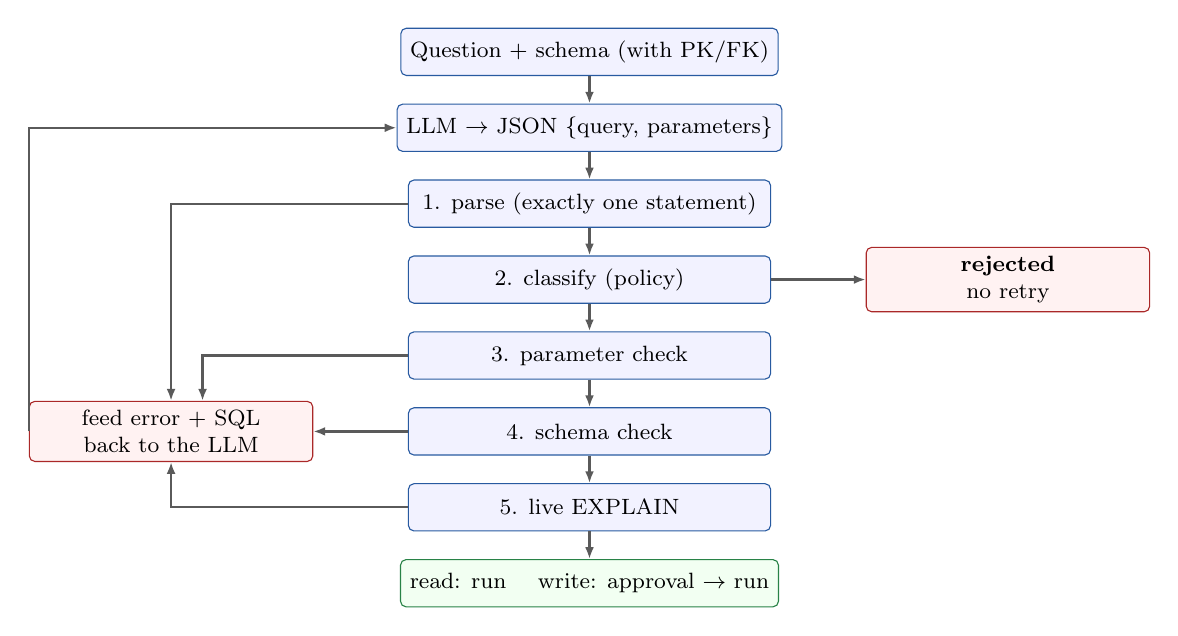
\begin{tikzpicture}[
  node distance=3.5mm,
  box/.style={rectangle, rounded corners=2pt, draw=panelblue, fill=blue!5,
              minimum width=4.6cm, minimum height=6mm, font=\footnotesize, align=center},
  bad/.style={rectangle, rounded corners=2pt, draw=panelred, fill=red!5,
              minimum width=3.6cm, minimum height=6mm, font=\footnotesize, align=center},
  arrow/.style={-{Latex[length=1.5mm]}, draw=panelgray, thick},
]
  \node[box] (q)   {Question + schema (with PK/FK)};
  \node[box, below=of q]   (llm) {LLM $\rightarrow$ JSON \{query, parameters\}};
  \node[box, below=of llm] (p)   {1. parse (exactly one statement)};
  \node[box, below=of p]   (c)   {2. classify (policy)};
  \node[box, below=of c]   (pa)  {3. parameter check};
  \node[box, below=of pa]  (s)   {4. schema check};
  \node[box, below=of s]   (l)   {5. live EXPLAIN};
  \node[box, below=of l, draw=panelgreen, fill=green!5] (x) {read: run \quad write: approval $\rightarrow$ run};
 
  \node[bad, right=12mm of c]  (rej) {\textbf{rejected}\\no retry};
  \node[bad, left=12mm of s]   (rep) {feed error + SQL\\back to the LLM};
 
  \foreach \a/\b in {q/llm, llm/p, p/c, c/pa, pa/s, s/l, l/x} \draw[arrow] (\a) -- (\b);
  \draw[arrow] (c) -- (rej);
  \draw[arrow] (p.west) -| (rep.north);
  \draw[arrow] (pa.west) -| ([xshift=4mm]rep.north);
  \draw[arrow] (s) -- (rep);
  \draw[arrow] (l.west) -| (rep.south);
  \draw[arrow] (rep.west) |- (llm.west);
\end{tikzpicture}
\end{center}
 
\begin{center}
\begin{tabular}{@{}l p{5.6cm} l l@{}}
\toprule
\textbf{Stage} & \textbf{Catches} & \textbf{Repairable?} & \textbf{File} \\
\midrule
\texttt{parser}     & syntax errors, 0 or 2+ statements        & yes & \texttt{sql/parser.py} \\
\texttt{policy}     & DDL off, dangerous functions, SELECT INTO, FOR UPDATE, nested writes, EXPLAIN ANALYZE & \textbf{no} & \texttt{sql/classifier.py} \\
\texttt{parameters} & missing values, \texttt{?} or \texttt{\$1}, \texttt{:x::int} & yes & \texttt{sql/params.py} \\
\texttt{schema}     & unknown tables or columns, ambiguous columns & yes & \texttt{sql/schema\_validator.py} \\
\texttt{live}       & anything PostgreSQL's planner rejects & yes & \texttt{sql/live\_validator.py} \\
\bottomrule
\end{tabular}
\end{center}
 
\keyidea{A \emph{mistake} is worth sending back to the model; a
\emph{forbidden request} is not. If the user asks to drop a table, asking the
model again just produces another DROP. Policy failures stop immediately with
status \texttt{rejected}.}
 
After validation there is one more policy check before any write reaches
the approval prompt: the unbounded-write guard (Section~\ref{sec:bounded}).
 
% =====================================================================
\section{Prompt design: giving the model the right context}
\label{sec:prompt}
 
The model can only use names it can see. v0.1 sent the schema as a JSON
dump of column types; the primary and foreign keys were collected but never
sent, so the model had to \emph{guess} how tables join.
v0.2 renders a compact, DDL-like text (\texttt{app/llm/prompts.py}):
 
\begin{lstlisting}
TABLE public.customers (id INTEGER PK, email VARCHAR(255), full_name VARCHAR(150), ...)
TABLE public.orders (id INTEGER PK, order_number VARCHAR(30), customer_id INTEGER, ...)
  FK (customer_id) -> public.customers(id)
  FK (shipping_address_id) -> public.addresses(id)
\end{lstlisting}
 
You can see exactly this text with the \texttt{show\_schema} command.
 
\subsection*{The rules in the system prompt, and why}
 
\begin{center}
\begin{tabular}{@{}p{6.4cm}p{8.2cm}@{}}
\toprule
\textbf{Rule} & \textbf{Reason} \\
\midrule
Exactly one statement, JSON only & the parser rejects anything else anyway; saying it up front saves retries \\
Only listed tables and columns; use the FKs for JOINs & fewer hallucinations, correct joins \\
Alias every table and prefix every column & avoids ambiguous-column errors \\
Every user value is a bind parameter \texttt{:p\_name} & no SQL injection; values are visible on the approval screen \\
Names start with \texttt{p\_} & \texttt{:limit} or \texttt{:order} are SQL keywords and can confuse the parser \\
\texttt{CAST(:p AS type)}, never \texttt{:p::type} & SQLAlchemy misreads \texttt{:p::type} \\
Explicit columns and a LIMIT for reads & small, readable results \\
UPDATE/DELETE need a WHERE on real columns & matches the policy that would reject them otherwise \\
If impossible, return \texttt{"query": ""} & ``I can't'' is better than inventing a table \\
\bottomrule
\end{tabular}
\end{center}
 
\subsection*{Few-shot example}
The prompt contains one worked example. It is labelled as an
\emph{illustrative} schema so the model does not copy its table names.
 
\subsection*{Reading the answer robustly}
Small local models often wrap JSON in code fences, write \texttt{"sql"}
instead of \texttt{"query"}, or return parameters as a list.
\texttt{parse\_llm\_payload()} in \texttt{app/llm/base.py} accepts all of
these. If the answer is still unusable, that counts as one attempt and the
model is told to answer with JSON only.
 
\subsection*{Model settings}
\begin{itemize}[leftmargin=*]
  \item \textbf{Temperature 0}: SQL generation should be deterministic.
  \item \textbf{Context size} (\texttt{OLLAMA\_NUM\_CTX=8192}): Ollama's default
        context can silently cut off a large schema; the model then invents
        the missing tables.
  \item \textbf{JSON mode} (\texttt{format: json} for Ollama,
        \texttt{response\_format=json\_object} for OpenAI).
\end{itemize}
 
% =====================================================================
\section{Defense in depth: three layers, not one}
 
``Defense in depth'' means stacking \emph{independent} controls so that a
single failure does not cause a breach.
 
\begin{enumerate}[leftmargin=*]
  \item \textbf{Static validation} in Python (parse, classify, parameters,
        schema, live \texttt{EXPLAIN}, unbounded-write guard).
  \item \textbf{Human approval} for every write, with one-time tokens.
  \item \textbf{Database permissions}: separate read-only and writer roles,
        and a read-only role that is read-only at the server.
\end{enumerate}
 
\begin{center}
\begin{tabular}{@{}p{4.4cm}p{5.4cm}p{4.4cm}@{}}
\toprule
\textbf{If this layer fails\dots} & \textbf{\dots this one still protects you} & \textbf{\dots and this one} \\
\midrule
Python validation has a bug & approval prompt                & read-only role refuses \\
Human approves a mistake    & row limit + rollback           & writer has no DDL rights \\
DBA grants too much         & Python never writes via the read connection & approval \\
\bottomrule
\end{tabular}
\end{center}
 
\keyidea{Defense in depth is not ``the same check three times''. It is three
checks with \emph{different} ways of failing.}
 
% =====================================================================
\section{Database permissions: the last line of defence}
 
\subsection*{Roles and grants}
\begin{lstlisting}[language=SQL]
CREATE ROLE sql_agent_readonly LOGIN PASSWORD '...';
GRANT USAGE ON SCHEMA public TO sql_agent_readonly;
GRANT SELECT ON ALL TABLES IN SCHEMA public TO sql_agent_readonly;
 
CREATE ROLE sql_agent_writer LOGIN PASSWORD '...';
GRANT SELECT, INSERT, UPDATE, DELETE ON ALL TABLES IN SCHEMA public
  TO sql_agent_writer;            -- no CREATE, DROP, ALTER, TRUNCATE
\end{lstlisting}
 
\subsection*{Default privileges}
\texttt{ALTER DEFAULT PRIVILEGES} decides what \emph{future} tables
inherit. Without it, tables created after the first \texttt{GRANT} are
invisible to the roles.
 
\subsection*{Read-only at three levels (v0.2)}
\begin{enumerate}[leftmargin=*]
  \item \textbf{Role setting}: \texttt{ALTER ROLE sql\_agent\_readonly SET
        default\_transaction\_read\_only = on} --- even a human using
        \texttt{psql} with this login gets read-only transactions.
  \item \textbf{Connection setting}: the read engine passes
        \texttt{-c default\_transaction\_read\_only=on}
        (\texttt{app/database/connection.py}).
  \item \textbf{Transaction}: every read starts with
        \texttt{SET TRANSACTION READ ONLY}.
\end{enumerate}
And underneath all three: the role simply has no \texttt{INSERT},
\texttt{UPDATE} or \texttt{DELETE} grant.
 
\subsection*{The startup guard}
\texttt{PermissionChecker.verify\_roles\_differ()} asks the database
\texttt{SELECT current\_user} on both connections and refuses to start if they
are the same role --- a misconfigured \texttt{.env} cannot silently remove
the separation.
 
% =====================================================================
\section{Parameters and approval tokens}
 
\subsection*{What parameterization is}
\begin{lstlisting}[language=SQL]
UPDATE products SET price = :p_price WHERE id = :p_id;
-- parameters: {"p_price": 39, "p_id": 7}
\end{lstlisting}
The driver sends values separately from the SQL text, so a value can never
become SQL syntax.
 
\subsection*{Parameter checks (\texttt{app/sql/params.py}, new in v0.2)}
\begin{center}
\begin{tabular}{@{}ll@{}}
\toprule
\textbf{Problem} & \textbf{Result} \\
\midrule
\texttt{:p\_city} used but no value given & error, sent back to the model \\
\texttt{?} or \texttt{\$1} placeholders   & error (SQLAlchemy needs named ones) \\
\texttt{:p\_date::date}                   & error: write \texttt{CAST(:p\_date AS date)} \\
a value that is a dict / object           & error \\
a value given but never used              & silently dropped \\
\bottomrule
\end{tabular}
\end{center}
 
Why is \texttt{:name::type} a problem? SQLAlchemy finds bind parameters with a
pattern like \texttt{:(\textbackslash w+)(?!:)} --- ``a name \emph{not}
followed by a colon''. For \texttt{:p\_date::date} the regex backtracks and
matches \texttt{:p\_dat}, leaving \texttt{e::date} behind. The SQL that
reaches PostgreSQL is broken.
 
\subsection*{Approval tokens bind the exact SQL}
After the human approves, \texttt{ApprovalManager.create\_token()} stores:
 
\begin{center}
\begin{tabular}{@{}ll@{}}
\toprule
\textbf{Field} & \textbf{Value} \\
\midrule
token       & 32 random bytes (\texttt{secrets.token\_urlsafe}) \\
sql\_hash   & SHA-256 of the exact query string \\
params\_hash& SHA-256 of the parameters as sorted-key JSON \\
\bottomrule
\end{tabular}
\end{center}
 
The executor calls \texttt{verify\_and\_consume()} before running anything:
the token is \emph{popped} (one-time use) and both hashes are recomputed from
the SQL and parameters the executor actually holds. One byte different
$\rightarrow$ refused. An approval for \texttt{price=39} can never run
\texttt{price=0}.
 
% =====================================================================
\section{Bounded writes}
\label{sec:bounded}
 
\subsection*{What counts as a WHERE}
\texttt{is\_potentially\_unbounded\_write()} in \texttt{app/sql/safety.py}:
 
\begin{lstlisting}[language=Python]
if not isinstance(tree, (exp.Update, exp.Delete)):
    return False
where = tree.args.get("where")          # the statement's OWN where
if where is None:
    return True                          # DELETE FROM orders
return where.find(exp.Column) is None    # WHERE 1 = 1, WHERE TRUE
\end{lstlisting}
 
\begin{center}
\begin{tabular}{@{}p{9.3cm}l@{}}
\toprule
\textbf{Statement} & \textbf{Verdict} \\
\midrule
\texttt{DELETE FROM orders WHERE id = :p\_id}                         & bounded \\
\texttt{DELETE FROM orders}                                           & rejected \\
\texttt{DELETE FROM orders WHERE 1 = 1}                               & rejected \\
\texttt{UPDATE p SET price = (SELECT max(price) FROM p WHERE id = 1)} & rejected \\
\texttt{DELETE FROM orders WHERE status = :p\_s} (500 rows match)     & bounded, but see below \\
\bottomrule
\end{tabular}
\end{center}
 
\subsection*{The row limit}
A WHERE can still match many rows. The executor runs the write inside a
transaction, reads \texttt{rowcount}, and if it is above
\texttt{MAX\_WRITE\_ROWS} it \textbf{rolls back}. The change never becomes
visible to anyone.
 
\subsection*{Statement and lock timeouts}
Writes run with \texttt{statement\_timeout} and \texttt{lock\_timeout} set
\emph{inside the transaction} (\texttt{set\_config(..., true)}), so a stuck
query or a locked row fails fast instead of hanging the agent.
 
% =====================================================================
\section{Human edits are untrusted input too}
\label{sec:edits}
 
At the approval prompt the user may choose \texttt{edit} and type new SQL.
In v0.1 the edited SQL was re-validated, but the unbounded-write check ran
only \emph{once}, before the first prompt. Typing
\texttt{DELETE FROM customers} as an edit and then approving deleted every
customer.
 
In v0.2 the write loop in \texttt{\_handle\_write()} re-runs \emph{every}
check on every iteration:
 
\begin{enumerate}[leftmargin=*]
  \item full validation (parse, policy, parameters, schema, live EXPLAIN);
  \item the edit must still be a write --- a SELECT typed at the approval
        prompt is refused, not silently run on the writer connection;
  \item the unbounded-write guard;
  \item a fresh approval prompt for the edited statement.
\end{enumerate}
 
\keyidea{Every input that can change what runs --- model output, human edits,
configuration --- goes through the same gate. ``The user typed it'' is not a
reason to skip a check.}
 
% =====================================================================
\section{Schema validation in detail}
 
\subsection*{Reads: let SQLGlot resolve every column}
\texttt{qualify()} rewrites the query so every column is attached to a
table, expands \texttt{SELECT *}, and raises if a column cannot be resolved.
The agent then checks every remaining \texttt{Table} node against the live
schema. CTE names and table functions such as \texttt{generate\_series()}
are skipped; cross-database names (\texttt{otherdb.public.t}) are rejected.
 
\subsection*{Identifier case}
PostgreSQL folds unquoted names to lower case:
\texttt{SELECT ID FROM Users} means \texttt{users.id}. v0.1 compared the raw
names and rejected that query. v0.2 normalises identifiers the same way
PostgreSQL does before comparing.
 
\subsection*{Writes: a simpler resolver}
For INSERT/UPDATE/DELETE the validator collects the tables and aliases and
checks each column against them. Special cases:
\begin{itemize}[leftmargin=*]
  \item \texttt{INSERT INTO t (a, b)}: \texttt{a} and \texttt{b} are
        \emph{identifiers}, not column nodes, so v0.1 never checked them.
        v0.2 does.
  \item \texttt{ON CONFLICT ... DO UPDATE SET x = EXCLUDED.x}:
        \texttt{EXCLUDED} is a PostgreSQL pseudo-table and is allowed.
  \item Columns that come from a CTE or sub-query alias are left to the
        live EXPLAIN check, which knows their real shape.
\end{itemize}
 
\subsection*{Why every column is registered as TEXT}
The validator only needs column \emph{names}. Real type strings (enums,
domains, arrays) can make SQLGlot's type parser fail, which would reject
valid queries for the wrong reason.
 
% =====================================================================
\section{Live validation with EXPLAIN, not EXPLAIN ANALYZE}
 
\begin{center}
\begin{tabular}{@{}lll@{}}
\toprule
\textbf{Command} & \textbf{Executes the query?} & \textbf{Allowed?} \\
\midrule
\texttt{EXPLAIN q}                         & No  & yes, used for validation \\
\texttt{EXPLAIN ANALYZE q} / \texttt{ANALYSE} & Yes & never \\
\bottomrule
\end{tabular}
\end{center}
 
\texttt{EXPLAIN} asks the planner ``how would you run this?''. It parses,
resolves names and types, checks privileges and builds a plan --- but touches
no rows. PostgreSQL accepts both spellings \texttt{ANALYZE} and
\texttt{ANALYSE}; v0.1 only blocked the first.
 
\subsection*{Reads}
Planned on the read-only connection.
 
\subsection*{Writes (new in v0.2)}
The read-only role has no UPDATE privilege, so it cannot even \emph{plan}
an UPDATE. Writes are therefore planned on the \textbf{writer} connection,
inside a transaction that is
\begin{enumerate}[leftmargin=*]
  \item started with \texttt{SET TRANSACTION READ ONLY},
  \item given a statement timeout,
  \item always \textbf{rolled back}.
\end{enumerate}
Plain EXPLAIN does not execute, and if it somehow did, the read-only
transaction would refuse and the rollback would undo it. The benefit: a
wrong column or type in an UPDATE is found \emph{before} the human is asked to
approve it, and the model gets a chance to fix it.
Switch it off with \texttt{LIVE\_VALIDATE\_WRITES=false}.
 
\subsection*{What EXPLAIN does not catch}
CHECK, UNIQUE and foreign-key violations, trigger behaviour, and races.
Those fail at execution time and the transaction rolls back --- for example
\texttt{delete customer 3} fails because customer 3 still has orders.
 
% =====================================================================
\section{The self-repair loop}
 
\begin{lstlisting}
You: show each customer's age
 
[attempt 1] LLM: SELECT c.full_name, c.age FROM customers c
            schema: Column 'age' could not be resolved
[attempt 2] the LLM receives:
              SQL: SELECT c.full_name, c.age FROM customers c
              Parameters: {}
              Problems: schema_validation: Column 'age' could not be resolved
            LLM: {"query": "", "explanation": "There is no age or birth date column."}
Agent: The request cannot be answered with the current schema. ...
\end{lstlisting}
 
\begin{center}
\begin{tabular}{@{}p{6.5cm}p{8.1cm}@{}}
\toprule
\textbf{Rule} & \textbf{Why} \\
\midrule
Send the failed SQL, not only the error & the model can fix its own query instead of starting over (new in v0.2) \\
Full validation on every attempt        & a fix for one problem can introduce another \\
Policy failures are not retried         & a forbidden request stays forbidden \\
Bad JSON from the model counts as an attempt & small models sometimes answer in prose \\
Bounded (\texttt{MAX\_SQL\_REPAIR\_ATTEMPTS}, default 2) & no infinite loops, no runaway cost \\
\bottomrule
\end{tabular}
\end{center}
 
% =====================================================================
\section{Execution details}
 
\subsection*{Reads (\texttt{DatabaseExecutor.execute\_read})}
\begin{enumerate}[leftmargin=*]
  \item \texttt{SET TRANSACTION READ ONLY} --- must be the first statement.
  \item \texttt{statement\_timeout} for this transaction only.
  \item The query runs with a \textbf{server-side cursor}
        (\texttt{stream\_results=True}) for plain SELECTs, so a million-row
        result is not pulled into memory just to keep the first
        \texttt{MAX\_RESULT\_ROWS}.
  \item It fetches \texttt{MAX\_RESULT\_ROWS + 1} rows: the extra row tells the
        agent the result was truncated.
\end{enumerate}
 
\subsection*{Writes (\texttt{execute\_write})}
\begin{enumerate}[leftmargin=*]
  \item Verify and consume the approval token.
  \item Set statement and lock timeouts.
  \item Execute, read \texttt{rowcount}; roll back if it is unknown or above
        \texttt{MAX\_WRITE\_ROWS}; otherwise commit.
  \item DDL (only if \texttt{ENABLE\_DDL=true}) has no row count, so it skips
        that check. In v0.1 DDL was always rolled back for that reason.
\end{enumerate}
 
\subsection*{Error messages}
SQLAlchemy wraps driver errors; the original is in \texttt{exc.orig}, which can
be \texttt{None}. v0.1 then printed the useless message \texttt{None}.
\texttt{db\_error\_message()} in \texttt{app/database/errors.py} falls back to
the wrapper and returns only the first line.
 
% =====================================================================
\section{Structured audit logging}
 
An audit log answers: \emph{who} asked \emph{what}, \emph{which} SQL was
generated, \emph{what} validation concluded, \emph{whether} it was approved,
and \emph{what} happened. The agent writes one JSON object per request to
\texttt{logs/audit.log} (JSONL), including rejected and failed requests.
 
\begin{lstlisting}
{"timestamp": "...", "request_id": "...", "mode": "execute",
 "natural_language_request": "change the price of product 7 to 39",
 "operation_type": "UPDATE", "sql": "UPDATE products SET price = :p_price WHERE id = :p_id",
 "tables": ["products"], "validation_result": "PASS",
 "approval_decision": "APPROVED", "execution_success": true, "affected_rows": 1,
 "error": null, "parameters": {"p_price": 39, "p_id": 7}}
\end{lstlisting}
 
Parameters whose \emph{name} looks secret (\texttt{password}, \texttt{token},
\texttt{api\_key}, \dots) are replaced by \texttt{***REDACTED***}.
Writing the log can never crash a request: errors while logging are ignored.
 
% =====================================================================
\section{Case studies: bugs found in v0.1}
\label{sec:cases}
 
Each bug below passed the original tests. Each one teaches a general lesson.
 
\begin{center}
\begin{tabular}{@{}p{4.3cm}p{5.2cm}p{5.1cm}@{}}
\toprule
\textbf{Bug} & \textbf{Root cause} & \textbf{Lesson} \\
\midrule
Edited SQL without WHERE was executed &
unbounded check ran before the edit loop, not inside it &
re-run every check after every change of input \\
\addlinespace
WHERE in a sub-query counted &
\texttt{tree.find(exp.Where)} searches the whole tree &
know whether you ask about the node or its descendants \\
\addlinespace
Dangerous functions allowed in writes &
denylist was checked only in the SELECT branch &
apply security checks before branching by type \\
\addlinespace
Write hidden in a CTE of a write &
nested-write check existed only for reads &
same as above \\
\addlinespace
\texttt{EXPLAIN ANALYSE} allowed &
string match on one spelling &
know your database's grammar \\
\addlinespace
OpenAI provider always failed &
strict structured output forbids \texttt{dict[str, Any]} &
test every provider at least once for real \\
\addlinespace
\texttt{INSERT} column names unchecked &
they are identifiers, not column nodes &
inspect the AST you actually get \\
\addlinespace
\texttt{SELECT ID FROM Users} rejected &
compared raw names, PostgreSQL folds case &
normalise like the database does \\
\addlinespace
Error message ``None'' &
\texttt{getattr(exc, "orig", exc)} when \texttt{orig} is \texttt{None} &
an attribute can exist and be empty \\
\addlinespace
DDL never succeeded &
DDL has \texttt{rowcount = -1}, treated as unknown &
one rule does not fit every statement type \\
\addlinespace
Wrong port in \texttt{.env.example} &
compose publishes 5433, example said 5432 &
documentation is code; test the quick-start \\
\bottomrule
\end{tabular}
\end{center}
 
% =====================================================================
\section{Reading the project code}
 
\begin{center}
\begin{tabular}{@{}p{5.2cm}p{9.4cm}@{}}
\toprule
\textbf{Concept} & \textbf{Where to look} \\
\midrule
Settings and validation       & \texttt{app/config.py} \\
Data models                   & \texttt{app/models.py} \\
Prompt and schema rendering   & \texttt{app/llm/prompts.py} \\
LLM interface + JSON parsing  & \texttt{app/llm/base.py} \\
Providers                     & \texttt{app/llm/ollama\_client.py}, \texttt{openai\_client.py}, \texttt{mock\_client.py} \\
Parsing                       & \texttt{app/sql/parser.py} \\
Classification (policy)       & \texttt{app/sql/classifier.py} \\
Parameter checks              & \texttt{app/sql/params.py} \\
Schema validation             & \texttt{app/sql/schema\_validator.py} \\
EXPLAIN probe                 & \texttt{app/sql/live\_validator.py} \\
Unbounded-write guard         & \texttt{app/sql/safety.py} \\
Schema introspection + cache  & \texttt{app/database/introspection.py}, \texttt{schema\_manager.py} \\
Execution                     & \texttt{app/database/executor.py} \\
Approval tokens               & \texttt{app/security/approval.py} \\
Role separation               & \texttt{app/security/permissions.py} \\
Audit log                     & \texttt{app/security/audit.py} \\
The pipeline                  & \texttt{app/agent.py} \\
CLI                           & \texttt{app/main.py} \\
\bottomrule
\end{tabular}
\end{center}
 
\textbf{Suggested reading order:} \texttt{models.py} $\rightarrow$
\texttt{parser.py} $\rightarrow$ \texttt{classifier.py} $\rightarrow$
\texttt{safety.py} $\rightarrow$ \texttt{params.py} $\rightarrow$
\texttt{schema\_validator.py} $\rightarrow$ \texttt{prompts.py} $\rightarrow$
\texttt{approval.py} $\rightarrow$ \texttt{executor.py} $\rightarrow$
\texttt{agent.py}. Read \texttt{tests/test\_hardening.py} next to each file:
every test there is a small, runnable example of one rule.
 
% =====================================================================
\section{Test yourself}
\label{sec:quiz}
 
Try to answer before reading the answer.
 
\begin{enumerate}[leftmargin=*, label=\textbf{Q\arabic*.}]
  \item The model returns \texttt{DROP TABLE orders}. How many times is the
        model called in total, and what status does the user see?
 
        \emph{Answer:} once; \texttt{rejected}. It is a policy failure, so
        there is no repair attempt.
 
  \item Why can't the live check plan an \texttt{UPDATE} on the read-only
        connection?
 
        \emph{Answer:} PostgreSQL checks privileges while planning, and the
        read-only role has no UPDATE privilege.
 
  \item The user approves \texttt{UPDATE products SET price = :p\_price WHERE
        id = :p\_id} with \texttt{p\_price = 39}. Could the executor run it
        with \texttt{p\_price = 0}?
 
        \emph{Answer:} no; the parameter hash in the token would not match.
 
  \item Is \texttt{DELETE FROM reviews WHERE rating < 3} allowed?
 
        \emph{Answer:} it is bounded (its WHERE references a column), so it
        reaches the approval prompt. If it matches more rows than
        \texttt{MAX\_WRITE\_ROWS}, it is rolled back after execution.
 
  \item Why does the prompt ask for parameter names like \texttt{:p\_limit}
        instead of \texttt{:limit}?
 
        \emph{Answer:} \texttt{limit} is a SQL keyword. Keywords used as
        placeholder names can confuse the parser; a fixed prefix avoids the
        whole class of problems.
 
  \item Name three independent reasons the read path cannot write.
 
        \emph{Answer:} no write grants on the role; the role's
        \texttt{default\_transaction\_read\_only}; the explicit
        \texttt{SET TRANSACTION READ ONLY}.
 
  \item The model wraps its answer in a markdown code fence and writes
        \texttt{\{"sql": "SELECT 1"\}}. What happens?
 
        \emph{Answer:} \texttt{parse\_llm\_payload} strips the fence, maps
        \texttt{sql} to \texttt{query}, and validation continues normally.
\end{enumerate}
 
% =====================================================================
\section{Further reading}
 
\begin{itemize}[leftmargin=*]
  \item PostgreSQL documentation: \emph{Privileges}, \emph{EXPLAIN},
        \emph{SET TRANSACTION}, \emph{Client Connection Defaults}.
  \item SQLGlot documentation: the expression tree, \texttt{qualify},
        dialects.
  \item OWASP: \emph{SQL Injection} and \emph{Query Parameterization} cheat
        sheets.
  \item OWASP: \emph{Top 10 for LLM Applications} (prompt injection,
        excessive agency).
  \item Saltzer and Schroeder (1975), \emph{The Protection of Information in
        Computer Systems} --- fail-safe defaults, least privilege.
  \item uv documentation: projects, lock files, dependency groups.
\end{itemize}
 
\end{document}
 